\documentclass[a4paper]{report}

\usepackage[T1]{fontenc}
\usepackage[utf8]{inputenc}
\usepackage[english]{babel}

\usepackage{booktabs}
\renewcommand{\arraystretch}{1.2}

% Display code - main interest is it can import external files
\usepackage{listings}
\usepackage[usenames]{xcolor}

% Custom style for the code
\lstset{
	commentstyle=\color{gray},
	tabsize=4,
	basicstyle={\small\ttfamily}
}

% TiKZ for the drawings
\usepackage{tikz}
\usetikzlibrary{shapes}

\setlength{\textwidth}{16cm} \setlength{\textheight}{23cm}
\setlength{\oddsidemargin}{0cm} % +0.5 si {\textwidth}{15cm} ; -0,5 si {\textwidth}{15cm}
\setlength{\headheight}{0cm} \setlength{\topmargin}{0.3cm}
\setlength{\headsep}{0cm}

\author{Clément Decoodt, Alexis Bauvin, Alexandre Janniaux}
\title{PR2 SE201: execution platforms}

\begin{document}

\maketitle

\section{Introduction}

In this report, we will detail our results on the analysis of MIPS code execution.

\section{Warm up}

Nothing to do here

\section{Pipeline}

There are many clues which show the processor is enabled to forwarding.

First, the statistics window tell us:
\begin{quote}
    ALU forwarded values: 2 (from execute: 2, memory stage: 0, write back: 0)
\end{quote}

Then, the log window tells us, for instruction 13:
\begin{quote}
    DEBUG [EXECUTE]: {FW} PC: 0x000011a0 forwarding changed value for ALU port A RS from: 0x0 to: 0xffffffe0
\end{quote}

But we can also tell that the processor does forward because of the pipeline window. 
Indeed, the processor compute the following instructions:

\begin{verbatim}
    1. nop
    2. addui r29,r29,-32
    3. sw 28(r29),r31
    4. sw 24(r29),r30
    5. or r30,r29,r0
\end{verbatim}

So instruction $3.$ and $4.$  depends on instruction $2.$ which is executed at cycle $12$. 
At instruction $13$, $12$ has been executed, but the result is not written back in register yet, 
and $3.$ is to be decoded. It means that $3.$ is able to use the result from $2.$ before $2.$ has finished
to store his value.
%TODO screenshot

\subsection{}

\subsection{}

\subsection{Multiplication and overflow}

\section{Processor design}

\subsection{Instruction set architecture}

We defined our architecture set instruction as the following:

\subsubsection{R-type instructions}

Instruction structure :

\begin{center}
	\begin{tabular}{|l|l|l|l|}
		\hline
		opcode & output register & input register 1 & input register 2 \\
		\hline
		7 bits & 3 bits & 3 bits & 3 bits \\
		\hline
	\end{tabular}
\end{center}

Instruction list :

\begin{center}
	\begin{tabular}{|l|l|l|}
		\hline
		Opcode & Mnemonic & Description \\
		\hline \hline
		\texttt{0000000} & \texttt{NOP} &  Does nothing \\
		\texttt{0000011} & \texttt{ADD} &  Adds two signed numbers \\
		\texttt{0000111} & \texttt{ADDU} & Adds two unsigned numbers \\
		\texttt{0000010} & \texttt{SUB} &  Substracts two signed numbers \\
		\texttt{0000110} & \texttt{SUBU} & Substracts two unsigned numbers \\
		\texttt{0000100} & \texttt{MULU} & Multiplied two unsigned numbers \\
		\hline
	\end{tabular}
\end{center}

Example:

\texttt{sub \$r1 \$r2 \$r3} : computes \texttt{\$r2} $-$ \texttt{\$r3} and stores the
result in \texttt{\$r1}. \\
Encodes to ${
	\underbrace{\texttt{0000010}}_{opcode}
	\underbrace{\texttt{001}}_{out}
	\underbrace{\texttt{010}}_{in 1}
	\underbrace{\texttt{011}}_{in 2}\mbox{}_2 % The mbox serves to add another subscript
}$ = \texttt{0x0453}$_{16}$

\subsubsection{I-type instructions}

Instruction structure :

\begin{center}
	\begin{tabular}{|l|l|l|}
		\hline
		opcode & output register & immediate value \\
		\hline
		2 bits & 3 bits & 11 bits \\
		\hline
	\end{tabular}
\end{center}

Instruction list :

\begin{center}
	\begin{tabular}{|l|l|l|}
		\hline
		Opcode & Mnemonic & Description \\
		\hline \hline
		\texttt{10} & \texttt{ADDIU} & Adds-accumulate an unsigned immediate
		                               value to output register \\
		\texttt{11} & \texttt{LWI} &   Copies the immediate value to
		                               the register \\
		\hline
	\end{tabular}
\end{center}

Example:

\texttt{addiu \$r6 420h} : computes \texttt{\$r6} $+$ \texttt{0x420} and stores
the result in \texttt{\$r6}. \\
Encodes to ${
	\underbrace{\texttt{10}}_{opcode}
	\underbrace{\texttt{110}}_{out}
	\underbrace{\texttt{10000100000}}_{value}\mbox{}_2
}$ = \texttt{0xb420}$_{16}$

\subsubsection{J-type instructions}

Instruction structure :

\begin{center}
	\begin{tabular}{|l|l|l|l|}
		\hline
		opcode & register 1 & register 2 & immediate value \\
		\hline
		4 bits & 3 bits & 3 bits & 6 bits \\
		\hline
	\end{tabular}
\end{center}

Instruction list :

\begin{center}
	\begin{tabular}{|l|l|l|}
		\hline
		Opcode & Mnemonic & Description \\
		\hline \hline
		\texttt{0010} & \texttt{LW} & Loads word from memory at address
		                              \texttt{\$r2 + immediate} (offset) into \\
		              &             & first register \\
		\texttt{0011} & \texttt{SW} & Stores word in \texttt{\$r1} to memory at
		                           address \texttt{\$r2 + immediate} (offset) \\
		\hline
	\end{tabular}
\end{center}

Example: if \texttt{\$r2} contains \texttt{0x1337},

\texttt{lw \$r1 \$r2 0x2a} : reads the word at address \texttt{\$r2} +
\texttt{0x2a} (i.e. \texttt{0x1361}) and stores it in \texttt{\$r1} \\
Encodes to ${
	\underbrace{\texttt{0010}}_{opcode}
	\underbrace{\texttt{001}}_{out}
	\underbrace{\texttt{010}}_{adr}
	\underbrace{\texttt{101010}}_{offset}\mbox{}_2
}$ = \texttt{0x22aa}$_{16}$

\subsubsection{K-type instructions}

Instruction structure :

\begin{center}
	\begin{tabular}{|l|l|l|l|}
		\hline
		opcode & immediate value & register 1 & register 2 \\
		\hline
		2 bits & 8 bits & 3 bits & 3 bits \\
		\hline
	\end{tabular}
\end{center}

Instruction list :

\begin{center}
	\begin{tabular}{|l|l|l|}
		\hline
		Opcode & Mnemonic & Description \\
		\hline \hline
		\texttt{01} & \texttt{BNE} & Jumps to \texttt{pc + immediate} if
		                             \texttt{\$r1 $\neq$ \$r2} \\
		\hline
	\end{tabular}
\end{center}

Example:

\texttt{bne -3h \$r1 \$r5} : compares \texttt{\$r1} and \texttt{\$r5} and
jumps to \texttt{\$pc + immediate} if they are different \\
Encodes to ${
	\underbrace{\texttt{01}}_{opcode}
	\underbrace{\texttt{11111101}}_{offset}
	\underbrace{\texttt{001}}_{reg 1}
	\underbrace{\texttt{101}}_{reg 1}\mbox{}_2
}$ = \texttt{0x7f4d}$_{16}$

\subsubsection{Instruction tree}

We are using a binary tree to determine the actual instruction :

\begin{center}
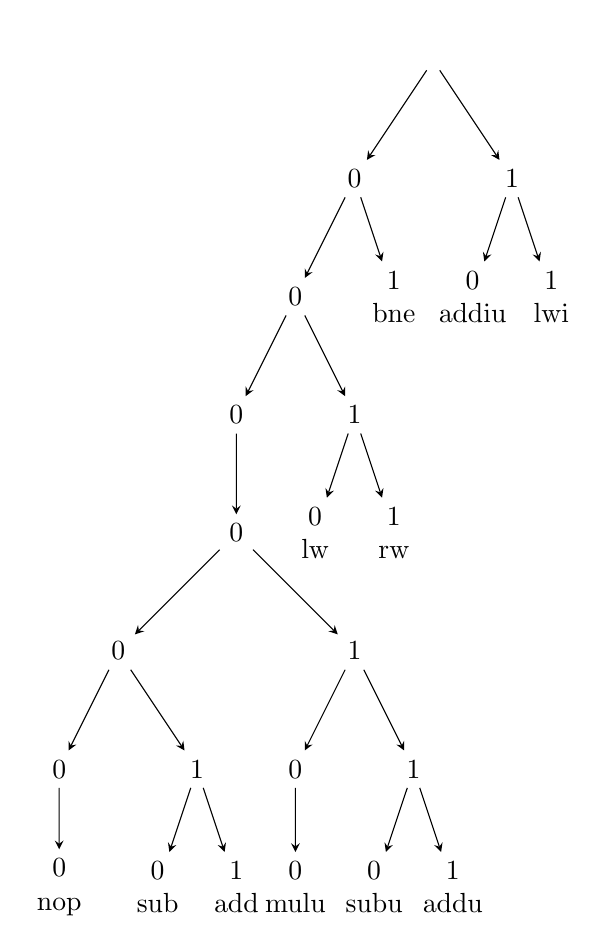
\begin{tikzpicture}[>=stealth]
	\tikzstyle{every node}=[align=center]
	\tikzstyle{level 1}=[sibling distance=20mm]
	\tikzstyle{level 2}=[sibling distance=10mm]
	\tikzstyle{level 4}=[sibling distance=10mm]
	\tikzstyle{level 5}=[sibling distance=30mm]
	\tikzstyle{level 6}=[sibling distance=20mm]
	\tikzstyle{level 7}=[sibling distance=10mm]
	\node {} [->]
		child {node {0}
			child[sibling distance=15mm] {node {0}
				child[sibling distance=15mm] {node {0}
					child {node {0}
						child {node {0}
							child[sibling distance=15mm] {node {0}
								child {node {0\\nop}}
							}
							child {node {1}
								child {node {0\\sub}}
								child {node {1\\add}}
							}
						}
						child {node {1}
							child[sibling distance=15mm] {node {0}
								child {node {0\\mulu}}
							}
							child[sibling distance=15mm] {node {1}
								child {node {0\\subu}}
								child {node {1\\addu}}
							}
						}
					}
				}
				child {node {1}
					child {node {0\\lw}}
					child {node {1\\rw}}
				}
			}
			child {node {1\\bne}}
		}
		child {node {1}
			child {node {0\\addiu}}
			child {node {1\\lwi}}
		}
	;
\end{tikzpicture}
\end{center}

\subsubsection{Assembly samples}

We will assume here that the assembler supports labels for the jumps -- which
the included Javascript one does.

\mbox{}\\
The following code will load the constant $2^{21}$ into the register
\texttt{\$r1} :
\lstinputlisting[language={[x86masm]Assembler}]{../src/two_pow_21.s}
To avoid the use of labels, it is equivalent to write \texttt{-2h} in
place of \texttt{loop} in the \texttt{bne} instruction.

\mbox{}\\
This is the correspondance between a bit of C code and its compiled
version :

% The tabular forces the codes to be on the same height
\noindent\begin{tabular}{cc}
	\begin{lstlisting}[language=C]
int *a = 0x200;
int s = 0;
for (int i = 0; i != 10; i++) {
	s = s + *a;
	a++;
}
\end{lstlisting}
	&
	\lstinputlisting[language={[x86masm]Assembler}]{../src/c_code.s}
\end{tabular}

\subsection{Pipelining}

\end{document}


